
%(BEGIN_QUESTION)
% Copyright 2011, Tony R. Kuphaldt, released under the Creative Commons Attribution License (v 1.0)
% This means you may do almost anything with this work of mine, so long as you give me proper credit

``Wet'' natural gas is mostly methane (CH$_{4}$) mixed with significant amounts of heavier hydrocarbon species such as ethane (C$_{2}$H$_{6}$), propane (C$_{3}$H$_{8}$), butane (C$_{4}$H$_{10}$), and pentane (C$_{5}$H$_{12}$).  A process for separating these heavier hydrocarbons from the chief component (methane) using compression and cooling is shown here:

$$\includegraphics[width=15.5cm]{i03084x01.eps}$$

Chilled gases enter the flash vessel, where methane rises and escapes in gaseous form, while all the other (heavier) hydrocarbon molecules condense into liquid and exit out the bottom.

\vskip 10pt

Suppose PT-115 is mis-calibrated, such that it falsely indicates a pressure lower than what is actually inside the flash vessel.  How will this mis-calibration affect the control of flash vessel pressure?  Will the operator be able to know anything is wrong by observing the DCS monitor screens for this process?

\vskip 20pt \vbox{\hrule \hbox{\strut \vrule{} {\bf Suggestions for Socratic discussion} \vrule} \hrule}

\begin{itemize}
\item{} Explain the purpose of the heat exchangers in this P\&ID, especially the two exchanging heat between the incoming (compressed) gas and the products coming off the top and bottom of the flash vessel.
\item{} Identify and explain the purpose of the ``PSV'' valve in this diagram.
\item{} Assuming air-to-open control valves, identify the correct actions for each loop controller (direct or reverse).
\item{} Identify the effect(s) of LV-108 failing shut.
\item{} Identify the effect(s) of PV-115 failing shut.
\end{itemize}

\underbar{file i03084}
%(END_QUESTION)





%(BEGIN_ANSWER)


%(END_ANSWER)





%(BEGIN_NOTES)

This mis-calibration will result in the actual flash vessel pressure being {\it greater} than it should be.

%INDEX% Control, proportional: proportional-only offset
%INDEX% Process: "wet" natural gas separation

%(END_NOTES)


